% --------------------------------------------------------------------
% Preamble
% --------------------------------------------------------------------
\documentclass[a4paper]{article}	

\usepackage[scaled]{helvet}
\renewcommand\familydefault{\sfdefault} 
\usepackage[T1]{fontenc}

% 'microtype' can only be used with pdflatex
\usepackage[protrusion=true,expansion=true]{microtype}
	
\usepackage[utf8]{inputenc}
\usepackage[english]{babel}
\usepackage{amsmath,amsfonts,amsthm,amssymb}
\usepackage{graphicx}
\usepackage{xcolor}

% Spacing between lines 
\usepackage{setspace}
\onehalfspacing

% ----- page layout 
\usepackage[
	a4paper,
	top=1in, bottom=1.25in, left=1.25in, right=1.25in
]{geometry}	

\setlength{\oddsidemargin}{5mm}			% Remove 'twosided' indentation
\setlength{\evensidemargin}{5mm}

\usepackage[
	colorlinks=true,
	urlcolor=magenta,
	linkcolor=blue, 	% [red]
%	anchorcolor 	 % [black]
	citecolor=black, 		% [green]
	filecolor=black, 	% [cyan]
	menucolor=black		% [red]
]{hyperref}

% Header and footer control
\usepackage{fancyhdr}
\setlength{\headheight}{15.2pt}
\pagestyle{fancy}

% ----- Table of contents 
\usepackage{titletoc}
\usepackage{tocloft}

\renewcommand\cftsecfont{\normalfont}
\renewcommand\cftsecpagefont{\normalfont}
\renewcommand{\cftsecleader}{\cftdotfill{\cftsecdotsep}}
\renewcommand\cftsecdotsep{\cftdot}
\renewcommand\cftsubsecdotsep{\cftdot}


% ----- Tables
\usepackage{booktabs}
\usepackage{colortbl}
\usepackage{longtable}
\usepackage{makecell}

% ----- Units formatting 
\usepackage{siunitx}

% ------ Macros for this document
\definecolor{yellowMSL}{RGB}{244,182,8}

% Mark-up for small changes (a few words only)
\newcommand{\proposed}[1]{{\color{cyan}{{#1}}}}
\newcommand{\deprecated}[1]{{\color{yellowMSL}{#1}}}

% Mark-up  for paragraphs. 
\usepackage{framed}
\newcommand{\proposedbox}[1]{
\colorlet{shadecolor}{gray!10}
{\color{cyan}\begin{shaded}
	{#1}
\end{shaded}}
}%

\newcommand{\deprecatedbox}[1]{
\colorlet{shadecolor}{gray!10}
{\color{yellowMSL}\begin{shaded}
	{#1}
\end{shaded}}
}%

% --------------------------------------------------------------------
% Front page definitions (do not change this)
% --------------------------------------------------------------------
\newcommand{\HRule}[1]{\rule{\linewidth}{#1}} 	% Horizontal rule

\makeatletter							% Title
\def\printtitle{%						
    {\centering \@title\par}}
\makeatother									

\makeatletter							% Author
\def\printauthor{%					
    {\raggedright \Large \@author}}				
\makeatother							


% --------------------------------------------------------------------
% Details of what to put on the front page (Change this)
% --------------------------------------------------------------------
\title{	\Large 
	\textsc{ Measurement Standards Laboratory of New Zealand } \\ [2.0cm]			
	\HRule{2pt} \\ [0.25cm]						
	\LARGE \textbf{\uppercase{Guidelines on Reporting and Publishing}}	\\% Title
    \Large \textit{A supplement to the MSL Quality Manual}
	\HRule{2pt} \\ [0.25cm]		
	\Large \today			
}

\author{
{\large 
	Text in this \proposed{colour} is awaiting approval by the 
	Quality Council.\\ 
	Text in this \deprecated{colour} is deprecated 
	and awaiting approval to be deleted.
} \\[\baselineskip]
 		
Measurement Quality Council\\	
Measurement Standards Laboratory of New Zealand\\	
}

% ----- Control over what will be included
\includeonly{
	general,
%	reports,
%	informal_reports,
%	electronic_reports,
%	copyright_and_licensing,
}

\begin{document}
\hypersetup{pageanchor=false}	% prevents a warning message
\fancyhf{}	% Header and footer are empty

% ------------------------------------------------------------------------------
% Title page
% ------------------------------------------------------------------------------
\thispagestyle{empty}		% Remove page numbering on this page
\pagestyle{plain}			% puts pages numbers back in front matter

\printtitle					% Print the title data as defined above
  	\vfill
\printauthor				% Print the author data as defined above
\newpage

\pagenumbering{roman}

\tableofcontents
\newpage

% ----- Main document now begins
\pagestyle{fancy}			% Turn on footer style control
\pagenumbering{arabic}
\hypersetup{pageanchor=true}
\setcounter{page}{1}		% Set page numbering to begin on this page

\fancyfoot[L]{Reporting and publishing}
\fancyfoot[C]{\today}
\fancyfoot[R]{Page \thepage\ of \pageref*{LastPage}}

\setlength{\parindent}{0cm}	% No indent when starting a new paragraph
\setlength{\parskip}{\baselineskip}	% Leave a blank line between paragraphs

% ----- These files contain the document content
\section{Numbers and units}
Numbers and units should be formatted following the NIST guide to the SI \cite{NIST_SI}.

Quantity values with units should not be split over lines. Use a non-breaking spacing to prevent this (in MS Word: CTRL-SHIFT-SPACE).

When numbers are expressed with more than four digits (either side of the decimal marker), a thin space is preferred to a coma, or nothing, as separator between groups of three digits. Some examples are shown in figure~\ref{fig:ex_number_formats} 
\begin{figure}[h]
\begin{center}
\begin{tabular}{Sl}
{do this} &  {not this} \\ \hline 
76483522 & 76,483,522 \\
43279.168 & 43,279.168 \\
8012 & 8,012 \\ 
18012 & 18,012 \\
0.4917223 & 0.4917223 
\end{tabular}
\caption{Preferred number formatting. Note that all numbers in the left-hand column are vertically aligned to the location of the decimal point.}
\label{fig:ex_number_formats}
\end{center}
\end{figure}

\subsection{Generating a space separator}
It is not easy to generate a thin space in Microsoft Word. The following recipe is one possibility:
\begin{enumerate}
\item Type a space normally (use a non-breaking space if needs be) 
\item Select the space and right click to obtain the context menu; select Font …
\item Select the Advanced tab and set Spacing to `Condensed' (the ``by 1 pt'' default is OK)
\item Click OK and copy the space to the clipboard 
\end{enumerate}

This thin space character can be pasted into numbers as required.

Using Microsoft Excel it is possible to select a normal-width space separator for groups of `thousands'  in the number formatting. Unfortunately, this does not insert spaces between groups of three digits to the right of the decimal marker. 

To set up Excel to insert a space between digits to the left of the decimal marker:
\begin{enumerate}
\item Find the `Use system separators' check box under `Editing Options' in the Excel Options menu 
\item Un-check this box and type a space character into the `Thousands Separator' box
\end{enumerate} 

Alternatively, to insert spaces between groups of three digits to the right of the decimal marker use a custom number format of ``\verb|#.### ### ###|''. Similarly, a custom number format of ``\verb|# ### ###|'' can be used to set a space as the thousands separator.

\section{Mathematical language}
Mathematical formulae and equations should be contained in complete English sentences with appropriate punctuation. 

Punctuation follows equations: a computation that ends a sentence needs to end with a full stop; otherwise an equation should be followed by a comma (an effective way to check for appropriate punctuation is to read text containing equations out loud). 

For example, the following sentence appears in a report for a transformer test set: 
\[
\text{For $\rho = \SI{-1}{\%}$ and $\varphi= \SI{1}{crad}$,\; }
\varepsilon = \frac{1-0.01}{\cos(0.01)} - 1 \; =\; \SI{-0.995}{\%}\,. 
\]

Often, the use of space and separate lines for equations can be helpful to a reader, as it is in this extract from a calibration report:
\begin{quote}

A comparator is used to evaluate the vector ratio $Q_\mathrm{X}/Q_\mathrm{N}$ where $Q_\mathrm{X}$ is the fundamental component of the signal vector at terminals X (either voltage or current) and $Q_\mathrm{N}$ is the fundamental component of the corresponding signal vector at terminals N. 

This ratio can be represented in polar co-ordinates as:
\[
\frac{Q_\mathrm{X}}{Q_\mathrm{N}} = (1 + \varepsilon) e^{\mathrm{j}\varphi} \;,
\]
where:

\begin{tabular}{rl}
$\varepsilon$ & is the ratio error, and \\
$\varphi$ & is the phase error, for the polar co-ordinate system. 
\end{tabular}

\vspace{\baselineskip}
This ratio can be also represented in rectangular co-ordinates as:
\[
\frac{Q_\mathrm{X}}{Q_\mathrm{N}} = 1 + \rho + \mathrm{j}\cdot\tan (\gamma) \;,
\]
where
\begin{tabular}{rl}
	$\rho$ &  is the ratio error, and \\
	$\tan (\gamma)$ & is the phase error, for the rectangular co-ordinate system. 
\end{tabular}

\vspace{\baselineskip}	
This ELTEL comparator reports the ratio error as $\rho$ (rectangular co-ordinate system) and the phase error as $\varphi$ (polar co-ordinate system).
\end{quote}

\subsection{Symbols and notation}
It is important to choose an appropriate set of symbols to represent quantities. That includes the alphabet, the font (Roman, bold, italic, etc) and the case. Getting the notion right can be hard: be prepared to spend more time on sorting this out than you might expect.

It pays to choose the style and a selection of symbols as early as possible when writing documents ( see~\S\ref{sss:style_guide} ). This may require careful consideration of what exactly will be described. Each symbol should only represent one thing, otherwise the intended meaning in your writing can become obscure and possibly ambiguous. 

Communicating efficiently with the reader is paramount: if there is an existing convention, follow it. Wherever possible, try to be consistent. If one document is closely related to another, then try to maintain consistent notation. 

\subsubsection{MSL style guide for symbols}
\label{sss:style_guide}
Here is a default guide for MSL publications. Follow this unless the rules are unsuitable for the work, or a distinct set of rules needs to be used (e.g., a scientific journal may ask for a specific style).

\begin{itemize}
\item Italicize symbols representing quantities or other variables (either Greek or Latin symbols). 

Abbreviated symbols, or full words, used as descriptors (often as subscripts or superscripts), should be in Roman font (not italics). For example, $V_\mathrm{input}$  (The `$V$' is italic, but not the subscript).

However, when variables, rather than descriptors or labels, appear in subscripts or superscripts they should be italicised. So, for example, the $i^\mathrm{th}$ instance of `$x$' could be written as $x_i$ (both `$x$' and `$i$' italicised).

\item Units and unit symbols should not be italicized, so $V_\mathrm{input}$ = \SI{12.1}{ V }.
	
\item Constants should be in Roman font. So, special symbols representing numbers, like $\mathrm{\pi}$, $\mathrm{e}$ and $\mathrm{i}$ or $\mathrm{j}$ (the imaginary unit), should be set in Roman font.
	
\item Operators should be set in Roman font. For instance, $\mathrm{d}y/\mathrm{d}x$ (the d's are in upright font).
	
\item Complex variables should use bold italic, such as $\bm{z}=\bm{x}+\mathrm{i} \bm{y}$. Some font families do not offer a bold italic font option, so this can be a problem.
	
\item Matrices and vectors should be written in bold Roman font.

\end{itemize}Note the equation editor in MS Word (or MathType, which is an extended commercial version) automatically applies some of these rules, but not all. 


\section{Scientific prose}
An excellent paper about the craft of writing scientific prose appeared in Scientific American in 1990 \cite{GopenAndSwan}. It develops seven structural principles that can be followed to make complicated scientific prose easier to read and understand. The principles are listed below as a convenient reminder, but the paper should be read to understand them properly.
\begin{enumerate}

\item	Follow a grammatical subject as soon as possible with its verb.
\item	Place in the stress position the ``new information'' you want the reader to emphasize (readers naturally emphasize material at the end of a sentence: this is the ``stress position'').
\item	Place the person or thing whose ``story'' a sentence is telling at the beginning of the sentence, in the topic position (information in the ``topic'' position usually begins a sentence and establishes a perspective for viewing the sentence as a unit). 
\item	Place appropriate ``old information'' (material already stated in the discourse) in the topic position for linkage backward and contextualization forward (when ``old'' information is continually placed in the topic position it helps the reader construct the logical flow of an argument). 
\item	Articulate the action of every clause or sentence in its verb. 
\item	In general, provide context for your reader before asking that reader to consider anything new. 
\item	In general, try to ensure that the relative emphases of the substance coincide with the relative expectations for emphasis raised by the structure.
\end{enumerate}

\subsection{Equations and prose in scientific documents}
David Mermin offered several simple principles about writing equations in scientific papers in his entertaining Reference Frame column in Physics Today \cite{Mermin}.
\begin{enumerate}

\item	Number all displayed equations (not just the ones you, the author, wish to refer to).
\item When referring to an equation, identify it by a phrase as well as a number (to help the reader remember what the equation was about).
\item	End a displayed equation with a punctuation mark (so the prose with equations embedded flows).

\end{enumerate}

\subsection{Tables}
As a general principle, use as little unnecessary decoration in tables as possible: it is the numbers or data that are of interest, not the graphic design. Tables should encourage the eye to compare data and help the reader to think about the information (rather than the design) being presented. 
Alignment is important when presenting numbers, because the eye picks up on vertical and horizontal patterns. If lines are drawn on a table, to frame or separate numbers, they can distract the reader from the data being presented. 
The following guidelines should be considered
\begin{itemize}
\item	Columns of decimal numbers should be aligned on the decimal point; columns of integers should be aligned on the right (the one's digit); text should usually be left-aligned.
\item	Draw as few horizontal and vertical lines as possible (consider using horizontal space instead of horizontal lines to separate blocks of information).
\item	Consider using captions to supplement column headings, by keeping column headings brief and putting extra details in the caption.
\item	The caption should be placed above the table. The caption text may use a smaller sized font than the many body and should be left-aligned.
\item	Units should be included in a column heading; unit symbols are preferred to full unit names, but be consistent.
\item	Use footnotes to convey information about specific entries in the table (e.g., entries that are out of scope).
\end{itemize}   
Table~\ref{tab:electrical_results} illustrates some of these guidelines.

\clearpage
\begin{sidewaysfigure}[h]
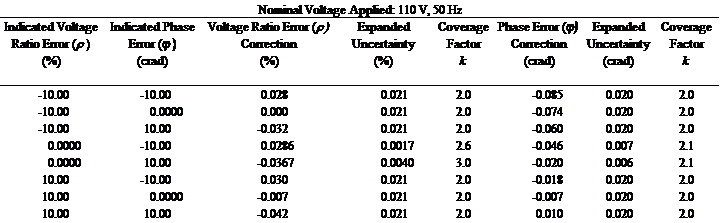
\includegraphics[width=\textwidth]{pictures/table_electrical_results}
\label{tab:electrical_results}
\caption{An example of tabulated measurement results. Note the vertical alignment of numbers and the caption above the table.}
\end{sidewaysfigure}
\clearpage

%\begin{table}[h]
%\centering
%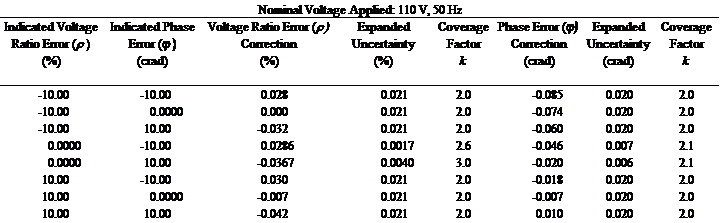
\includegraphics[scale=.7]{pictures/table_electrical_results}
%\label{tab:electrical_results}
%\caption{An example of tabulated measurement results. Note the vertical alignment of numbers and the caption above the table.}
%\end{table}

\subsection{Uncertainty}
Clear statements about measurement uncertainty and related concepts are sadly lacking in the metrology literature. This is a problem, because readers are presented with jargon that is rarely helpful to them. Often too, it seems that poor style is self-perpetuating. Presumably because authors do not have clear stylistic guidelines available and are unclear in their own minds about the subject. 

MSL should adopt a clear style when writing about uncertainty. These notes help avoid common problems.

\paragraph{Which uncertainty?}
Often, the intended meaning of `uncertainty' is not clear. Statements like ``all measurements have uncertainties'' may be used without a reasonable definition in the surrounding context.

There are two specific types of uncertainty: standard uncertainty and expanded uncertainty. It is better to write the full term, which, as a side-effect, will also discourage any tendency to be glib (``all measurements have standard uncertainties'' just doesn't have the same ring to it). 

\paragraph{What is uncertain?}
A measurement result (measured value) is never uncertain: this is a known number, call it $y$, which may be read from an instrument or calculated from data. Uncertainty only occurs when $y$ is used in place of the measurand (call that $Y$). The uncertainty is then about what happens when the value $y$ is used instead of $Y$. 

To write clearly and use the word uncertainty correctly, a useful trick is to replace `the uncertainty of $y$' in a sentence with `the uncertainty of $y$ as an estimate of $Y$'. (If overdone, this may become rather laborious, but, this form should be used unless the reader will understand the writer's intention from clear statements made close by in the text.) 

\paragraph{Prefer the word `error'} 
Measurement error is the difference between the measurand $Y$ and the measured value $y$. All measurements are subject to measurement error (we never expect that $y=Y$). So, while it is unhelpful to say something like ``all measurements have uncertainties'', what we could say is that ``all measurements are subject to measurement error''.

\paragraph{Measured values are estimates; values of uncertainty are calculated}

One often reads that uncertainty has been estimated. This is used in many authoritative works, but it is unhelpful and should be avoided. The term ``estimate'' should be reserved for a measurement result (as an estimate of the measurand). 

Measurement is a process that produces an estimate of a measurand. This is fundamental. When we talk about the uncertainty in a result, as an estimate of the measurand, we generally intend that the uncertainty is calculated according to a common set of rules (GUM). 

The verbs `measure' and `estimate' are synonymous from our perspective. Although, `measure' is preferred to `estimate', this does not justify the use of `estimate' to describe calculations of uncertainty.  

So, for instance, don't write
\begin{quote}
``This uncertainty was estimated by …'',
\end{quote}
instead write
\begin{quote}
``This expanded uncertainty was calculated by …''.
\end{quote}
There is a reason for writing  `estimating uncertainty' in authoritative works, but it is rather specialised and unhelpful to most metrologists (which is why we discourage this usage). The GUM associates a Gaussian distribution with the error generated by a measurement procedure. The standard deviation of this  distribution is not known. However, the standard uncertainty associated with a result can be considered an estimate of the actual standard deviation. This is analogous to the distinction made in statistics between a sample standard deviation and a population standard deviation. Note, however, that the GUM method for calculating expanded uncertainty deals with this inherent imprecision (by using statistical tables of Student-$t$). So, there is no need to bring it to the reader's attention by using the word `estimate'.

Another reason for discouraging expressions like `estimating uncertainty' is that it implies there is some actual `true' value of `uncertainty', which is misleading. Granted, one might, in the GUM context, claim to estimate the standard uncertainty of the Gaussian distribution of measurement error–--a statistical parameter that is presumed to exist. However, it is often the expanded uncertainty that is referred to as being `estimated' and an expanded uncertainty need not be associated with any unique physical parameter.

\paragraph{Level of Confidence}
The level of confidence associated with a statement of expanded uncertainty is often said to be estimated. This too should be avoided. For instance,
\begin{quote}
``The expanded uncertainties were calculated using a coverage factor $k = 2.1$ and define an interval estimated to have a \SI{95}{\%} level of confidence''
\end{quote}
would be better expressed as
\begin{quote}
``The expanded uncertainties were calculated using a coverage factor $k = 2.1$, for a \SI{95}{\%} level of confidence''.
\end{quote}
The use of `estimated' above may reflect the author's reticence to claim a level of confidence of precisely \SI{95}{\%}. If that is so, then a suitable phrase might be ``for a level of confidence of at least \SI{95}{\%}''. 

Note that the author's reticence is of no value to the reader of a report. The essential information is that the GUM process has been followed using a coverage factor $k$ of definite value. The reader may wish to calculate the standard uncertainty, so the report must provide enough information to do this: it this case by dividing the value of expanded uncertainty by the reported value of $k$.

\paragraph{Coverage factor and degrees of freedom}
The reader will need to know the number of degrees of freedom associated with the standard uncertainty of a measurement if they intend to carry out uncertainty calculations of their own. 

Sometimes a value of coverage factor is described as being `derived from the Student-$t$ distribution'. This is not very helpful. Consider instead reporting both the coverage factor and the number of degrees of freedom associated with the standard uncertainty of the measurement.

It is certainly true that statistical tables for the Student-$t$ distribution can be consulted, or a computer programme used, to obtain the number of degrees of freedom corresponding to a coverage factor. However, the author has this information already and can provide it directly; there is no need to mysteriously refer to a \textit{`derivation from the Student-$t$ distribution'} and expect the reader to reverse-engineer the calculation. 

\paragraph{The colloquial meaning of uncertainty}
A thing that is uncertain is not accurately known. So, a measurand may correctly be described to be uncertain. 

However, things that are unpredictable may also be described as uncertain, such as the weather. A measurand is not uncertain in this sense, because it is considered fixed. This is an important point and the source of confusion: never suggest that the measurand is variable or, worse, random. 

The unpredictability of a measurement result is associated with the inevitability of measurement error (the difference between the measured value and the measurand). So, measurement error may be correctly described as uncertain, in that it is both unknown and random.

There are two specific technical terms: expanded uncertainty and standard uncertainty. One is associated with uncertainty about a measurand and the other with an unpredictable measurement error. An expanded uncertainty is the half-width of an interval that is likely to cover the actual measurand. A standard uncertainty, on the other hand, is an estimate of the standard deviation of the Gaussian distribution of measurement error.

It is important not to confuse these two concepts.

\paragraph{The purpose of measurement}
Measurements are always performed for a reason: they inform decisions by providing information about the physical world. 

The correctness of any decision based on measurement results will be uncertain, because the corresponding measurands cannot be known exactly. This is where uncertainty about a measurand affects human activity; it is where the colloquial meaning of uncertainty applies to measurement. 

For instance, a decision must be be made between two possible actions: A or B. The decision will be based on the level of some quantity $X$, which is measured. Four possible outcomes depend on how the measured value $x$ compares with some fixed value $Y$: 
\begin{enumerate}[label=\roman*)]
\item A is correctly chosen, 
\item A is incorrectly chosen, 
\item B is correctly chosen, and 
\item B is incorrectly chosen.
\end{enumerate} 
Incorrect decisions can arise because of measurement error. Any decision process should be designed to minimise the occurrence of bad decisions, but they may occur nevertheless. 

When writing for a general audience, it is important to consider the link between the world of measurements and the world that we live in. This is surely the fundamental reason for paying any attention to uncertainty, yet it is rarely acknowledged. 

\section{Metrological reports}
Every page of the report shall use \SI{25}{mm} left, right, top and bottom page margins, unless this is impractical, and paragraph spacing should be single, except where otherwise stated. 
 
Paragraphs within the body text shall be separated by a single blank line and have no indentation.

Headings within the body text shall be followed by a 1.5-line width vertical space. The body text will follow immediately on the next line, without indentation.

\subsection{Printing and binding}
All paper report pages shall be printed single-sided.  The front page will use one of the standard MSL report front covers (see below), normal white paper will be used for the body of the report. A clear cover will be placed over the front page and an MSL report back cover will be added after the last page. The report will be bound using a white binder clip.

\subsection{Report covers}
 \label{ss:report_covers}
There are several MSL report front covers: use the one that gives the highest level of endorsement possible to ALL the reported results – any exception must be approved by the Chief Metrologist or Quality Manager.

\begin{itemize}
\item	A plain report cover for calibration, test or verification reports of measurements that are not covered by MSL's IANZ accreditation;
\item	An IANZ-endorsed \textit{calibration laboratory} cover for calibration reports of measurements that are included in MSL's IANZ accreditation, but not included in the CMCs in the BIPM database;
\item	An IANZ- and BIPM-endorsed \textit{calibration laboratory} cover for reports of measurements included in MSL's IANZ accreditation as well as the CMCs in the BIPM database;
\item	An IANZ-endorsed \textit{laboratory} cover for test or verification reports of measurements included in MSL's IANZ applied physics accreditation scope.
\end{itemize}

Note that when an endorsed report is being issued that contains some results outside the current scope of accreditation, the text under the IANZ logo must be:
\begin{quote}
\textit{All measurements reported herein, unless otherwise noted, have been performed in accordance with the laboratory's scope of accreditation.}
\end{quote}

\paragraph{Issuing body and traceability statement}
All covers include the following statements:

\begin{quote}\begin{minipage}{.7\textwidth}
ISSUED BY: \\
\textbf{Measurement Standards Laboratory of New Zealand} \\[\baselineskip]
Established under the Measurement Standards Act 1992 and\\
the National Standards Regulations 2019 to provide uniform\\ 
measurement of physical quantities throughout New Zealand.\\

All results quoted in this report are directly traceable to the\\
national measurement standards held by the Measurement\\ 
Standards Laboratory of New Zealand (MSL). MSL is New\\ 
Zealand's national metrology institute and operates within\\ 
Callaghan Innovation.
\end{minipage}\end{quote}

\subsection{Front page}
The front (cover) page:
\begin{itemize}
\item	must have ``Page 1 of [number of pages]'' printed in the top left-hand corner in bold;
\item	may have a job reference directly below the page number in bold;
\item	must have a title, which should be about one-third distance down the page and left aligned in bold;
\item	may have an identification for the instrument(s), e.g. serial number, either as part of the title or elsewhere on the front page;
\item	must have a report number that follows the title after two blank lines; 
The report number format is left-aligned and in bold font: register name/calendar year (yyyy)/sequential number (obtained from section report register), followed by report date; e.g. Temperature/2009/853, 21 January 2009.
\end{itemize}

\subsection{Header and footer on subsequent pages}
There will be a 2-line header, with: 
\begin{itemize}
\item	``Measurement Standards Laboratory of New Zealand'' centred and printed in bold on the first line; 
\item	in the second line, the report number and date are aligned to the left margin, and the page number [of pages] is aligned to the right margin;
\item	there should be 1.5-line width spacing between the lines.
\end{itemize}
The footer will contain the following warning about copying; the text will be centred, in italic, and use two lines (see also Appendix 1 in IANZ Procedures and conditions of accreditation \cite{IANZ_PC}): 
\begin{quote}
\centering\textit{This report may not be reproduced, except in full, without the written consent of the Chief Metrologist, Measurement Standards Laboratory of New Zealand.}
\end{quote}

\subsection{Second page}
The body of the second page begins with four blank lines followed by the report title, in bold, followed by another blank line.

\subsection{Signature page}
The last page of the main body of the report contains the signatures, as described below. Note, the signatures page does not have to be the last page of the report. Appendices, such as drawings, graphs or tables may be included following the signatures page.

The signatures page of the report shall be signed by the workers who contributed to the report, the checker who reviewed it and the Chief Metrologist (or delegate) who authorizes it. These individuals shall also initial all other pages of paper reports, but this not required for electronic reports.

For IANZ-endorsed reports, at least one of the workers or the checker signing the report must be a \deprecated{recognised IANZ signatory for the measurement class(es)} \proposed{Key Technical Person for the technical procedure(s)}  covering the measurements.

The person signing as Chief Metrologist, or for the Chief Metrologist, must be identified as such:  for the Chief Metrologist, use the label ``Chief Metrologist''; for a delegate use ``for Chief Metrologist''.

It is not necessary to identify the function of everyone signing the report.\footnote{This was a requirement under 17025:2005, but not in 17025:2017.}  However, a title (such as ``Technical Officer'', ``Scientist'', ``Electrical Metrologist'') and/or a subject area descriptor (e.g., photometry, temperature, etc.) may be used.

If a worker or checker is unable to sign the report, approval must be sought from that individual before signing \textit{per persona} (p.p.). A record of that approval must be kept with the job file.

\subsection{Report structure}
The report body may include the following headings, where relevant:
\begin{quote}
\begin{tabbing}
\textbf{Description}\hspace{12mm}\=including manufacturer (either a list or a proper sentence)\\[\baselineskip]

\textbf{Identification}\mbox{}\\[\baselineskip]

\textbf{Client}\mbox{}\\[\baselineskip]

\textbf{Date(s) of Test or Date(s) of Calibration}\mbox{}\\[\baselineskip]

\textbf{Objective}\mbox{}\\[\baselineskip]

\textbf{Method}\mbox{}\\[\baselineskip]

\textbf{Conditions}\mbox{}\\[\baselineskip]

\textbf{Results}\mbox{}\\[\baselineskip]

\textbf{Notes}\mbox{}\\[\baselineskip]

\textbf{Uncertainty}\mbox{}\\[\baselineskip]


\textbf{Conclusion}\>\begin{minipage}[t]{.7\textwidth}
(statements of fact only, such as verification of compliance with a documentary standard or regulation)\\[\baselineskip]
For example:\\

This gauge complies with the accuracy requirements of BS1780:1985\\ or an industrial gauge. (Paragraph 7.2.1 of BS1780: 1985 requires\\ hat the error in pressure indication shall not exceed \SI{1}{\%} of the\\ 
maximum scale value at any point above \SI{10}{\%} and below \SI{90}{\%} of the \\
maximum scale value, i.e. an error of \SI{36}{psi} in this case. The error\\ 
over the rest of the scale shall not exceed \SI{1.5}{\%} of the maximum scale\\ 
value, i.e. an error of \SI{54}{psi}.)\\

or\\

The measured mass values of these weights lie within the maximum\\ 
permissible limits for Class M1 as stated in IOML International \\
Recommendation No. 20. 

\end{minipage}
\end{tabbing}
\end{quote}

The report shall state the number of the technical procedure used, including the version number, for example: ``The weights were compared against reference standards of known mass and density following procedure MSLT.M.001.005.''  This reference may be contained, for instance, in a section entitled Technical Procedure, or in the Method section.

\subsection{Re-issued reports}
Clause 7.8.8.1 of 17025:2017 requires that any change of information in re-issued reports be clearly identified and, where it is appropriate, the reason for the change should be given. We offer some guidance on how to do this here, however, other approaches may be acceptable.
\begin{enumerate}
\item	A new page can be inserted as page 2 of the report. This will contain a section titled ``Reissue Statement'' and identify the changes. The reason for inserting a whole new page is that it may avoid changes to the page layout of the original report (although pages numbers will be different).
\item	A decision about how to identify the changes needs to be made. When considering this question, assume that the client will not need to identify the difference between the old and new reports on more than one occasion. So, avoid over-highlighting changes. Nevertheless, it may be appropriate to tag or otherwise highlight individual changes embedded in other details. 
\end{enumerate}
The following is an example.

\textbf{\large Reissue Statement}\\

This report has been re-issued with the following changes:
\begin{enumerate}
\item	In the header of pages 2 to 8, the year incorrectly given as 2018 (but the year on title page 1 was correct).  The original date in the header is now written as ``27 May \sout{2018} 2019'' and the date of re-issue has been added.  
\item	The units reported in the first column of Table 1, Table 2 and the Table of Uncertainties of the original report were reported as mm. The correct units are inch. 
\item	Some values in Table 1 were incorrect. Values that have changed are indicated by a double dagger symbol $\ddagger$ (unicode 2021 – type 2021, then press alt-X), for example $0.93\,\ddagger$.
\item	There is a grammatical error in the final paragraph of page 4 (`include' has been changed to `includes').
\end{enumerate}  

\subsection{Fonts}
\subsubsection{Microsoft Word}
In Microsoft Word, the following fonts should be used.

On the front page, the Arial Narrow font is used, and all text is in bold. The sizes are as follows:
\begin{itemize}
\item	page number and job reference are set in 12-point, 
\item	the title is set in 18-point, and 
\item	the report number is set in 16-point.
\end{itemize}
The header and footer on all subsequent pages use 10-point Times New Roman font. The first line of the header is in bold; the warning in the footer about copying is in italic. 

The title on the second page uses Arial Narrow font and is set in 16-point bold.

In the main body of the report, the headings use Arial Narrow font and are set in 14-point bold. The body text uses 11-point Times New Roman font.
 
The Symbol font should be used as appropriate.

\subsubsection{Other text processors}
The Arial typeface has licensing terms that prohibit free redistribution, so the Arial font family is not always available on text processing systems. There are however, look-a-likes that provide satisfactory alternatives.

\subsection{Out-of-scope results (IANZ and CIPM MRA CMCs)}
It is acceptable to issue an IANZ-endorsed report that contains a small proportion of results outside the MSL accredited scope. In such cases, the text on the report cover under the IANZ logo must indicate that not all results are within scope (see \S\ref{ss:report_covers}) and the out-of-scope results must be clearly identified in the report (e.g., by adopting a distinctive notation or highlighting). If the out-of-scope nature relates to smaller uncertainties claimed, the report should also indicate a value of uncertainty that would be within scope.

It is acceptable to issue a report with the CIPM MRA logo containing a small proportion of results that are not covered by CMCs published in the Appendix C section of the BIPM key comparison database (KCDB). Those items shall be clearly identified as not being supported by the CIPM MRA (e.g., by adopting a distinctive notation or using a grey background on tables or figures).

\subsection{Informal reporting of measurements}
On rare occasions, MSL may report measurements without fully applying the procedures of the quality system. 

Such reporting must be authorized by the Chief Metrologist.

One situation where informal reporting may be acceptable is in the context of scientific collaboration, which might ultimately result in publication of MSL measurements. Another possibility is during the manufacturing of a product, where early detection of deviations from design targets may be very helpful.

Informal reporting may lighten the overhead associated with issuing MSL calibration reports. Nevertheless, quality principles should still be applied (checking of technical procedure and data, traceability to the SI, etc).

The purpose of this policy is to protect clients, and MSL, from any undesirable outcomes arising from incorrect use of data that has been provided informally. Our quality system is intended to eliminate mistakes. Bypassing that system increases the risk that data contains errors. MSL trades on its reputation. The reputational risk to MSL, of a mistake being associated with our work, must be considered and discussed with the Chief Metrologist.

All data provided informally shall be accompanied by a disclaimer notice. This notice shall make clear that MSL does not stand by the quality of the data provided, which should not be used to inform critical decisions. 

A template for the disclaimer follows. This text may be adapted to different situations (words in bold font between square brackets can be modified appropriately, the other text in square brackets may be used, or modified, if appropriate). The final text must be approved by the Chief Metrologist.

\begin{quote}
\textit{The [\textbf{data reported on}] is provided `as is', without warranty of any kind, to [\textbf{recipient}] for [\textbf{purpose}] only. [{The data shall not be made publicly available, nor provided to a third party, without the consent of the MSL Chief Metrologist.}] [The data should not be used to inform any critical decisions.] This disclaimer must accompany any copies of the data.}
\end{quote}

\subsection{Electronic reports}
An electronic report can be viewed on screen, or printed, by a client. We assume here that an electronic report is a PDF file representing a calibration report. 

The format of an electronic report must comply with the same general report formatting guidelines given in this document. 

The cover page will include one of the standard MSL report covers as a background image (watermark).

Electronic reports are produced by word-processing software (Word, LaTeX, etc), but electronic signatures are added to the PDF report in a distinct part of the report publication process, using different software. The two parts-–-production and signing-–-must be handled separately. 
 
This section describes how to: 
\begin{itemize}
\item	add an MSL report cover to the background of a cover page in a Word document, and
\item	how to add electronic signatures to a PDF report, and 
\item	how to calculate a numerical code for a particular file, which can be used to verify the integrity of file later.
\end{itemize}

\subsubsection{How to add an MSL report cover in Word}
\begin{enumerate}
\item	The cover page and the body of the report should be created as different Word ``sections''. 

This can be done by creating a new document and on the first page inserting a Next Page section break from the Breaks dropdown list on the Layout tab.
\item 	The MSL report cover image should be loaded as a custom Watermark from the design tab (figure~\ref{fig:word_watermark_dialog}). Select the \SI{100}{\%} scaling and uncheck the washout tick box. Then select and load the image file (accept to work off-line, if prompted).
\begin{figure}[h]
\centering
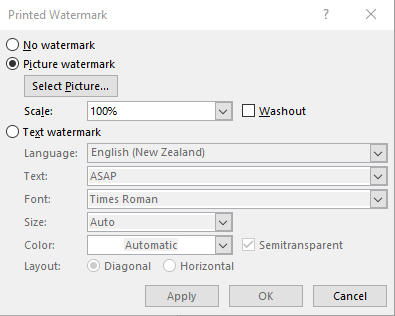
\includegraphics[scale=1]{pictures/word_watermark_dialog}
\caption{Word dialog box for adding a watermark.}
\label{fig:word_watermark_dialog}
\end{figure}
\item	The watermark will appear a bit washed out on the screen; don't worry, that's just to remind you it is in the background. 

However, the watermark will appear on every page-–-read on. 
\item Open the header of the first body page (not the cover page) by double clicking in the header region. Then, deselect the ``Link to Previous'' button on the Header and Footer tab. 

Select the background image and delete it. The image on the cover page will remain. (If the ``Link to Previous'' button is disabled, you can go ahead and delete the background image on the first page.)

\end{enumerate}

\subsubsection{Signing an electronic report}
A signature image can be placed in a PDF file using \href{https://acrobat.adobe.com/nz/en/acrobat/pdf-reader.html}{Adobe Acrobat Reader DC}.
\begin{enumerate}
\item Open the PDF report file with the Reader. Select the ``Fill \& Sign'' option from the tools available (may be visible on the right, or else in the Tools menu)
\begin{center}

\includegraphics[scale=1]{pictures/acrobat_signing}
\end{center}
\item Select the ``Fill and sign'' option, when presented with the choice:
\begin{center}
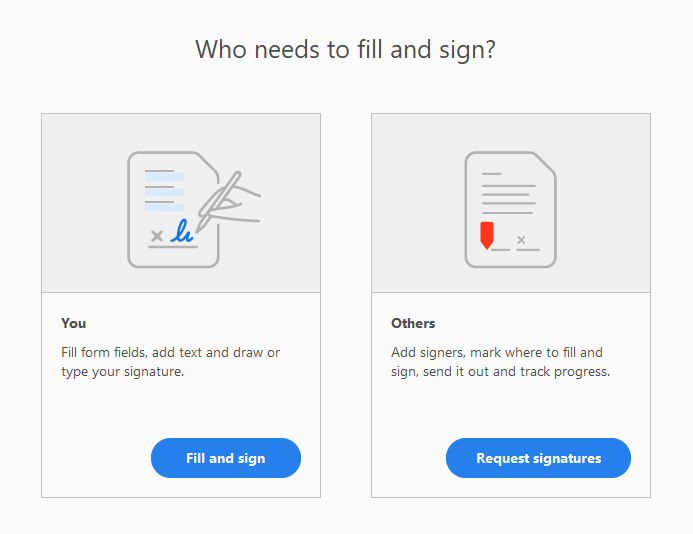
\includegraphics[scale=.6]{pictures/acrobat_signing_2}
\end{center}
\item A signing tool bar appears: 
\begin{center}

\includegraphics[scale=1]{pictures/acrobat_signing_3}
\end{center}
Go to the signature page of the report and click on the fountain pen icon, marked ``sign''. 

If it is the first time the Reader software is being used, you will need to load a signature file. Otherwise the software will present you with the image used last time. 
\item Click on the signature then place it in the document. A simple menu allows you to resize the image afterwards, if necessary. 
\begin{center}

\includegraphics[scale=.6]{pictures/acrobat_signing_4}
\end{center}
\item Save the file.
\end{enumerate}

\subsection{Checking the integrity of a report file}
Under 17025, there is a responsibility to manage the integrity of documents. Errors can occur during transmission of electronic records. It is also possible to edit PDFs with some software.

One way to prove that a file has not been changed is to use an \href{http://en.wikipedia.org/wiki/Md5sum}{MD5 checksum}. This is a code (a hexadecimal number) that can be calculated for any file. By keeping a record of the MD5 code of the signed report, we can check the integrity of a file later (e.g., after being emailed to a client). 

A checksum can be calculated in the Windows console, using the command ``CertUtil''. Here is an example:
\begin{center}

\includegraphics[scale=.6]{pictures/md5_cmd}
\end{center}
The command takes the form: 
\begin{quote}
\texttt{
> CertUtil -hashfile "\textit{Windows file path}" md5}
\end{quote}
The checksum result is the number \texttt{6c818093080a8d5b7c2cab72d738d8f5}.
 
There are many ways to calculate a checksum. Here is a simple Python script that takes a file path as input argument on the command line and prints the checksum (wil work in Python 2 or 3):

\begin{center}
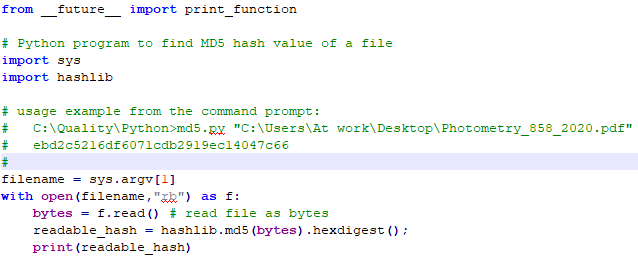
\includegraphics[scale=.8]{pictures/md5_python}
\end{center}

\section{Copyright and licensing}
Copyright is a property right that exists in certain original works. With few exceptions, copyright exists in original works created by government agencies just as it does in original works created by others. A licence (that is, permission) is needed to reuse most government copyright works because, without one, a person will infringe copyright in a work when he or she does any of a number of ``restricted acts''. The most common restricted act is copying the work or a substantial part of it.

Creative Commons licences are freely available copyright licences that enable the reuse of copyright works in a standardised way. Creative Commons is an international organisation with affiliate organisations around the world. Information about the New Zealand affiliate organisation can be found at \cite{CCNZ}. 

The New Zealand Government Open Access and Licensing framework (NZGOAL) \cite{NZGOAL} provides guidance for government agencies to follow when releasing copyright works and non-copyright material for re-use by others. NZGOAL seeks to foster a culture of sharing of government material and encourages the licensing of government copyright works for re-use using Creative Commons New Zealand law.
 
The Creative Commons licence below is likely to be the most appropriate for MSL publications. Called ``Attribution-NoDerivs 3.0 New Zealand'', the licence allows a document to be redistributed for any purpose, even commercially. Modifications to the work are not permitted, nor is it permitted in any way to suggest that the licensor endorses the use of the material. 

When using Word, there is a Microsoft add-on for Office that makes it easy to insert a license (unfortunately, however, the spelling of ``licence'' is American).

It may be helpful to summarise the nature of the licence in a few words, especially when a document is printed, making on-line access more difficult. Here is an example that was created using the Creative Commons logo and a text editor.
\begin{center}
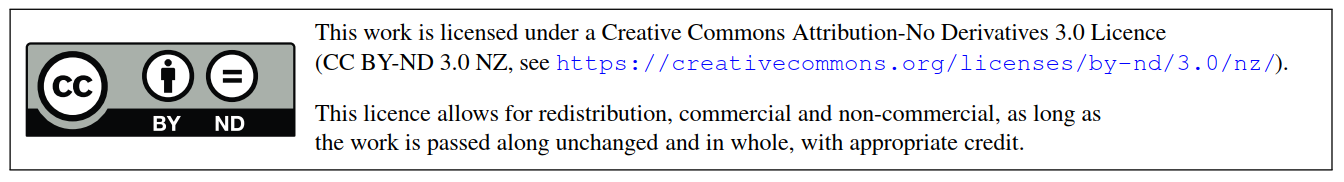
\includegraphics[scale=.41]{pictures/cc_license}
\end{center}

When using LaTeX, there is a Creative Commons license included in the style files for MSL Technical Guides and company reports.
\section{Metrological reports}
Every page of the report shall use \SI{25}{mm} left, right, top and bottom page margins, unless this is impractical, and paragraph spacing should be single, except where otherwise stated. 
 
Paragraphs within the body text shall be separated by a single blank line and have no indentation.

Headings within the body text shall be followed by a 1.5-line width vertical space. The body text will follow immediately on the next line, without indentation.

\subsection{Printing and binding}
All paper report pages shall be printed single-sided.  The front page will use one of the standard MSL report front covers (see below), normal white paper will be used for the body of the report. A clear cover will be placed over the front page and an MSL report back cover will be added after the last page. The report will be bound using a white binder clip.

\subsection{Report covers}
 \label{ss:report_covers}
There are several MSL report front covers: use the one that gives the highest level of endorsement possible to ALL the reported results – any exception must be approved by the Chief Metrologist or Quality Manager.

\begin{itemize}
\item	A plain report cover for calibration, test or verification reports of measurements that are not covered by MSL's IANZ accreditation;
\item	An IANZ-endorsed \textit{calibration laboratory} cover for calibration reports of measurements that are included in MSL's IANZ accreditation, but not included in the CMCs in the BIPM database;
\item	An IANZ- and BIPM-endorsed \textit{calibration laboratory} cover for reports of measurements included in MSL's IANZ accreditation as well as the CMCs in the BIPM database;
\item	An IANZ-endorsed \textit{laboratory} cover for test or verification reports of measurements included in MSL's IANZ applied physics accreditation scope.
\end{itemize}

Note that when an endorsed report is being issued that contains some results outside the current scope of accreditation, the text under the IANZ logo must be:
\begin{quote}
\textit{All measurements reported herein, unless otherwise noted, have been performed in accordance with the laboratory's scope of accreditation.}
\end{quote}

\paragraph{Issuing body and traceability statement}
All covers include the following statements:

\begin{quote}\begin{minipage}{.7\textwidth}
ISSUED BY: \\
\textbf{Measurement Standards Laboratory of New Zealand} \\[\baselineskip]
Established under the Measurement Standards Act 1992 and\\
the National Standards Regulations 2019 to provide uniform\\ 
measurement of physical quantities throughout New Zealand.\\

All results quoted in this report are directly traceable to the\\
national measurement standards held by the Measurement\\ 
Standards Laboratory of New Zealand (MSL). MSL is New\\ 
Zealand's national metrology institute and operates within\\ 
Callaghan Innovation.
\end{minipage}\end{quote}

\subsection{Front page}
The front (cover) page:
\begin{itemize}
\item	must have ``Page 1 of [number of pages]'' printed in the top left-hand corner in bold;
\item	may have a job reference directly below the page number in bold;
\item	must have a title, which should be about one-third distance down the page and left aligned in bold;
\item	may have an identification for the instrument(s), e.g. serial number, either as part of the title or elsewhere on the front page;
\item	must have a report number that follows the title after two blank lines; 
The report number format is left-aligned and in bold font: register name/calendar year (yyyy)/sequential number (obtained from section report register), followed by report date; e.g. Temperature/2009/853, 21 January 2009.
\end{itemize}

\subsection{Header and footer on subsequent pages}
There will be a 2-line header, with: 
\begin{itemize}
\item	``Measurement Standards Laboratory of New Zealand'' centred and printed in bold on the first line; 
\item	in the second line, the report number and date are aligned to the left margin, and the page number [of pages] is aligned to the right margin;
\item	there should be 1.5-line width spacing between the lines.
\end{itemize}
The footer will contain the following warning about copying; the text will be centred, in italic, and use two lines (see also Appendix 1 in IANZ Procedures and conditions of accreditation \cite{IANZ_PC}): 
\begin{quote}
\centering\textit{This report may not be reproduced, except in full, without the written consent of the Chief Metrologist, Measurement Standards Laboratory of New Zealand.}
\end{quote}

\subsection{Second page}
The body of the second page begins with four blank lines followed by the report title, in bold, followed by another blank line.

\subsection{Signature page}
The last page of the main body of the report contains the signatures, as described below. Note, the signatures page does not have to be the last page of the report. Appendices, such as drawings, graphs or tables may be included following the signatures page.

The signatures page of the report shall be signed by the workers who contributed to the report, the checker who reviewed it and the Chief Metrologist (or delegate) who authorizes it. These individuals shall also initial all other pages of paper reports, but this not required for electronic reports.

For IANZ-endorsed reports, at least one of the workers or the checker signing the report must be a \deprecated{recognised IANZ signatory for the measurement class(es)} \proposed{Key Technical Person for the technical procedure(s)}  covering the measurements.

The person signing as Chief Metrologist, or for the Chief Metrologist, must be identified as such:  for the Chief Metrologist, use the label ``Chief Metrologist''; for a delegate use ``for Chief Metrologist''.

It is not necessary to identify the function of everyone signing the report.\footnote{This was a requirement under 17025:2005, but not in 17025:2017.}  However, a title (such as ``Technical Officer'', ``Scientist'', ``Electrical Metrologist'') and/or a subject area descriptor (e.g., photometry, temperature, etc.) may be used.

If a worker or checker is unable to sign the report, approval must be sought from that individual before signing \textit{per persona} (p.p.). A record of that approval must be kept with the job file.

\subsection{Report structure}
The report body may include the following headings, where relevant:
\begin{quote}
\begin{tabbing}
\textbf{Description}\hspace{12mm}\=including manufacturer (either a list or a proper sentence)\\[\baselineskip]

\textbf{Identification}\mbox{}\\[\baselineskip]

\textbf{Client}\mbox{}\\[\baselineskip]

\textbf{Date(s) of Test or Date(s) of Calibration}\mbox{}\\[\baselineskip]

\textbf{Objective}\mbox{}\\[\baselineskip]

\textbf{Method}\mbox{}\\[\baselineskip]

\textbf{Conditions}\mbox{}\\[\baselineskip]

\textbf{Results}\mbox{}\\[\baselineskip]

\textbf{Notes}\mbox{}\\[\baselineskip]

\textbf{Uncertainty}\mbox{}\\[\baselineskip]


\textbf{Conclusion}\>\begin{minipage}[t]{.7\textwidth}
(statements of fact only, such as verification of compliance with a documentary standard or regulation)\\[\baselineskip]
For example:\\

This gauge complies with the accuracy requirements of BS1780:1985\\ or an industrial gauge. (Paragraph 7.2.1 of BS1780: 1985 requires\\ hat the error in pressure indication shall not exceed \SI{1}{\%} of the\\ 
maximum scale value at any point above \SI{10}{\%} and below \SI{90}{\%} of the \\
maximum scale value, i.e. an error of \SI{36}{psi} in this case. The error\\ 
over the rest of the scale shall not exceed \SI{1.5}{\%} of the maximum scale\\ 
value, i.e. an error of \SI{54}{psi}.)\\

or\\

The measured mass values of these weights lie within the maximum\\ 
permissible limits for Class M1 as stated in IOML International \\
Recommendation No. 20. 

\end{minipage}
\end{tabbing}
\end{quote}

The report shall state the number of the technical procedure used, including the version number, for example: ``The weights were compared against reference standards of known mass and density following procedure MSLT.M.001.005.''  This reference may be contained, for instance, in a section entitled Technical Procedure, or in the Method section.

\subsection{Re-issued reports}
Clause 7.8.8.1 of 17025:2017 requires that any change of information in re-issued reports be clearly identified and, where it is appropriate, the reason for the change should be given. We offer some guidance on how to do this here, however, other approaches may be acceptable.
\begin{enumerate}
\item	A new page can be inserted as page 2 of the report. This will contain a section titled ``Reissue Statement'' and identify the changes. The reason for inserting a whole new page is that it may avoid changes to the page layout of the original report (although pages numbers will be different).
\item	A decision about how to identify the changes needs to be made. When considering this question, assume that the client will not need to identify the difference between the old and new reports on more than one occasion. So, avoid over-highlighting changes. Nevertheless, it may be appropriate to tag or otherwise highlight individual changes embedded in other details. 
\end{enumerate}
The following is an example.

\textbf{\large Reissue Statement}\\

This report has been re-issued with the following changes:
\begin{enumerate}
\item	In the header of pages 2 to 8, the year incorrectly given as 2018 (but the year on title page 1 was correct).  The original date in the header is now written as ``27 May \sout{2018} 2019'' and the date of re-issue has been added.  
\item	The units reported in the first column of Table 1, Table 2 and the Table of Uncertainties of the original report were reported as mm. The correct units are inch. 
\item	Some values in Table 1 were incorrect. Values that have changed are indicated by a double dagger symbol $\ddagger$ (unicode 2021 – type 2021, then press alt-X), for example $0.93\,\ddagger$.
\item	There is a grammatical error in the final paragraph of page 4 (`include' has been changed to `includes').
\end{enumerate}  

\subsection{Fonts}
\subsubsection{Microsoft Word}
In Microsoft Word, the following fonts should be used.

On the front page, the Arial Narrow font is used, and all text is in bold. The sizes are as follows:
\begin{itemize}
\item	page number and job reference are set in 12-point, 
\item	the title is set in 18-point, and 
\item	the report number is set in 16-point.
\end{itemize}
The header and footer on all subsequent pages use 10-point Times New Roman font. The first line of the header is in bold; the warning in the footer about copying is in italic. 

The title on the second page uses Arial Narrow font and is set in 16-point bold.

In the main body of the report, the headings use Arial Narrow font and are set in 14-point bold. The body text uses 11-point Times New Roman font.
 
The Symbol font should be used as appropriate.

\subsubsection{Other text processors}
The Arial typeface has licensing terms that prohibit free redistribution, so the Arial font family is not always available on text processing systems. There are however, look-a-likes that provide satisfactory alternatives.

\subsection{Out-of-scope results (IANZ and CIPM MRA CMCs)}
It is acceptable to issue an IANZ-endorsed report that contains a small proportion of results outside the MSL accredited scope. In such cases, the text on the report cover under the IANZ logo must indicate that not all results are within scope (see \S\ref{ss:report_covers}) and the out-of-scope results must be clearly identified in the report (e.g., by adopting a distinctive notation or highlighting). If the out-of-scope nature relates to smaller uncertainties claimed, the report should also indicate a value of uncertainty that would be within scope.

It is acceptable to issue a report with the CIPM MRA logo containing a small proportion of results that are not covered by CMCs published in the Appendix C section of the BIPM key comparison database (KCDB). Those items shall be clearly identified as not being supported by the CIPM MRA (e.g., by adopting a distinctive notation or using a grey background on tables or figures).

\subsection{Informal reporting of measurements}
On rare occasions, MSL may report measurements without fully applying the procedures of the quality system. 

Such reporting must be authorized by the Chief Metrologist.

One situation where informal reporting may be acceptable is in the context of scientific collaboration, which might ultimately result in publication of MSL measurements. Another possibility is during the manufacturing of a product, where early detection of deviations from design targets may be very helpful.

Informal reporting may lighten the overhead associated with issuing MSL calibration reports. Nevertheless, quality principles should still be applied (checking of technical procedure and data, traceability to the SI, etc).

The purpose of this policy is to protect clients, and MSL, from any undesirable outcomes arising from incorrect use of data that has been provided informally. Our quality system is intended to eliminate mistakes. Bypassing that system increases the risk that data contains errors. MSL trades on its reputation. The reputational risk to MSL, of a mistake being associated with our work, must be considered and discussed with the Chief Metrologist.

All data provided informally shall be accompanied by a disclaimer notice. This notice shall make clear that MSL does not stand by the quality of the data provided, which should not be used to inform critical decisions. 

A template for the disclaimer follows. This text may be adapted to different situations (words in bold font between square brackets can be modified appropriately, the other text in square brackets may be used, or modified, if appropriate). The final text must be approved by the Chief Metrologist.

\begin{quote}
\textit{The [\textbf{data reported on}] is provided `as is', without warranty of any kind, to [\textbf{recipient}] for [\textbf{purpose}] only. [{The data shall not be made publicly available, nor provided to a third party, without the consent of the MSL Chief Metrologist.}] [The data should not be used to inform any critical decisions.] This disclaimer must accompany any copies of the data.}
\end{quote}

\subsection{Electronic reports}
An electronic report can be viewed on screen, or printed, by a client. We assume here that an electronic report is a PDF file representing a calibration report. 

The format of an electronic report must comply with the same general report formatting guidelines given in this document. 

The cover page will include one of the standard MSL report covers as a background image (watermark).

Electronic reports are produced by word-processing software (Word, LaTeX, etc), but electronic signatures are added to the PDF report in a distinct part of the report publication process, using different software. The two parts-–-production and signing-–-must be handled separately. 
 
This section describes how to: 
\begin{itemize}
\item	add an MSL report cover to the background of a cover page in a Word document, and
\item	how to add electronic signatures to a PDF report, and 
\item	how to calculate a numerical code for a particular file, which can be used to verify the integrity of file later.
\end{itemize}

\subsubsection{How to add an MSL report cover in Word}
\begin{enumerate}
\item	The cover page and the body of the report should be created as different Word ``sections''. 

This can be done by creating a new document and on the first page inserting a Next Page section break from the Breaks dropdown list on the Layout tab.
\item 	The MSL report cover image should be loaded as a custom Watermark from the design tab (figure~\ref{fig:word_watermark_dialog}). Select the \SI{100}{\%} scaling and uncheck the washout tick box. Then select and load the image file (accept to work off-line, if prompted).
\begin{figure}[h]
\centering
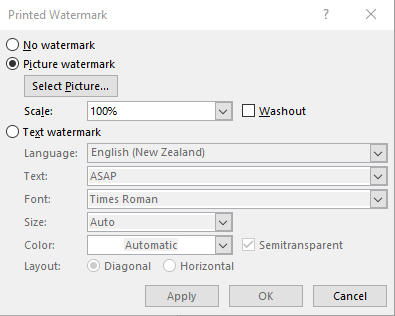
\includegraphics[scale=1]{pictures/word_watermark_dialog}
\caption{Word dialog box for adding a watermark.}
\label{fig:word_watermark_dialog}
\end{figure}
\item	The watermark will appear a bit washed out on the screen; don't worry, that's just to remind you it is in the background. 

However, the watermark will appear on every page-–-read on. 
\item Open the header of the first body page (not the cover page) by double clicking in the header region. Then, deselect the ``Link to Previous'' button on the Header and Footer tab. 

Select the background image and delete it. The image on the cover page will remain. (If the ``Link to Previous'' button is disabled, you can go ahead and delete the background image on the first page.)

\end{enumerate}

\subsubsection{Signing an electronic report}
A signature image can be placed in a PDF file using \href{https://acrobat.adobe.com/nz/en/acrobat/pdf-reader.html}{Adobe Acrobat Reader DC}.
\begin{enumerate}
\item Open the PDF report file with the Reader. Select the ``Fill \& Sign'' option from the tools available (may be visible on the right, or else in the Tools menu)
\begin{center}

\includegraphics[scale=1]{pictures/acrobat_signing}
\end{center}
\item Select the ``Fill and sign'' option, when presented with the choice:
\begin{center}
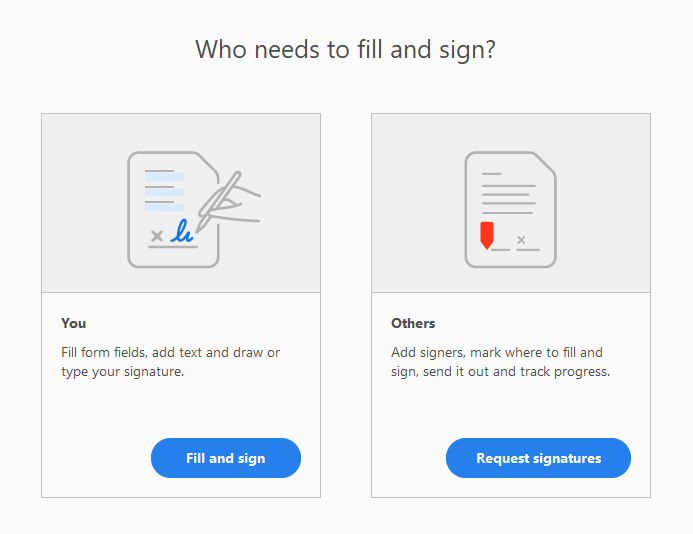
\includegraphics[scale=.6]{pictures/acrobat_signing_2}
\end{center}
\item A signing tool bar appears: 
\begin{center}

\includegraphics[scale=1]{pictures/acrobat_signing_3}
\end{center}
Go to the signature page of the report and click on the fountain pen icon, marked ``sign''. 

If it is the first time the Reader software is being used, you will need to load a signature file. Otherwise the software will present you with the image used last time. 
\item Click on the signature then place it in the document. A simple menu allows you to resize the image afterwards, if necessary. 
\begin{center}

\includegraphics[scale=.6]{pictures/acrobat_signing_4}
\end{center}
\item Save the file.
\end{enumerate}

\subsection{Checking the integrity of a report file}
Under 17025, there is a responsibility to manage the integrity of documents. Errors can occur during transmission of electronic records. It is also possible to edit PDFs with some software.

One way to prove that a file has not been changed is to use an \href{http://en.wikipedia.org/wiki/Md5sum}{MD5 checksum}. This is a code (a hexadecimal number) that can be calculated for any file. By keeping a record of the MD5 code of the signed report, we can check the integrity of a file later (e.g., after being emailed to a client). 

A checksum can be calculated in the Windows console, using the command ``CertUtil''. Here is an example:
\begin{center}

\includegraphics[scale=.6]{pictures/md5_cmd}
\end{center}
The command takes the form: 
\begin{quote}
\texttt{
> CertUtil -hashfile "\textit{Windows file path}" md5}
\end{quote}
The checksum result is the number \texttt{6c818093080a8d5b7c2cab72d738d8f5}.
 
There are many ways to calculate a checksum. Here is a simple Python script that takes a file path as input argument on the command line and prints the checksum (wil work in Python 2 or 3):

\begin{center}
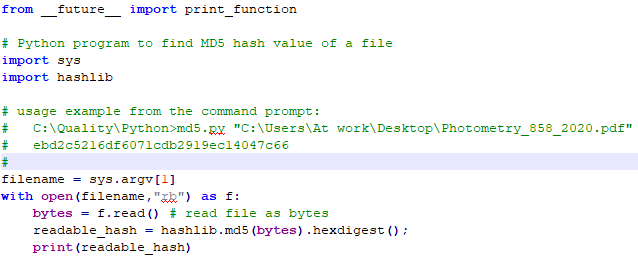
\includegraphics[scale=.8]{pictures/md5_python}
\end{center}


\include{informal_reports}
\include{electronic_reports}
\section{Copyright and licensing}
 \label{s_copyright}
Copyright is a property right that exists in certain original works. With few exceptions, copyright exists in original works created by government agencies just as it does in original works created by others. A licence (that is, permission) is needed to reuse most government copyright works because, without one, a person will infringe copyright in a work when he or she does any of a number of ``restricted acts''. The most common restricted act is copying the work or a substantial part of it.

Creative Commons licences are freely available copyright licences that enable the reuse of copyright works in a standardised way. Creative Commons is an international organisation with affiliate organisations around the world. Information about the New Zealand affiliate organisation can be found at \cite{CCNZ}. 

The New Zealand Government Open Access and Licensing framework (NZGOAL) \cite{NZGOAL} provides guidance for government agencies to follow when releasing copyright works and non-copyright material for re-use by others. NZGOAL seeks to foster a culture of sharing of government material and encourages the licensing of government copyright works for re-use using Creative Commons New Zealand law.
 
The Creative Commons licence below is likely to be the most appropriate for MSL publications. Called ``Attribution-NoDerivs 3.0 New Zealand'', the licence allows a document to be redistributed for any purpose, even commercially. Modifications to the work are not permitted, nor is it permitted in any way to suggest that the licensor endorses the use of the material. 

When using Word, there is a Microsoft add-on for Office that makes it easy to insert a license (unfortunately, however, the spelling of ``licence'' is American).

It may be helpful to summarise the nature of the licence in a few words, especially when a document is printed, making on-line access more difficult. Here is an example that was created using the Creative Commons logo and a text editor.
\begin{center}
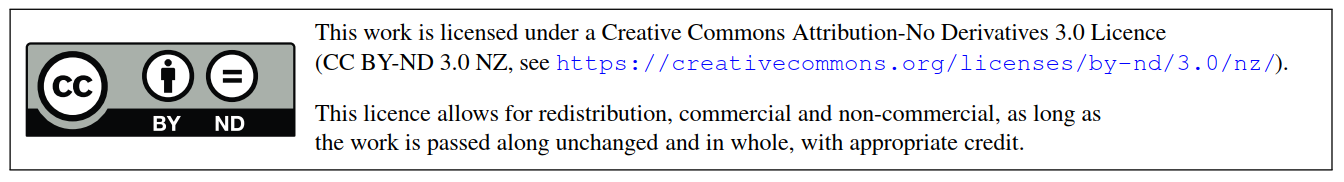
\includegraphics[scale=.41]{pictures/cc_license}
\end{center}

When using LaTeX, there is a Creative Commons license included in the style files for MSL Technical Guides and company reports.

\appendix	% Changes the style of the headings for sections
% \section{Abbreviations}
\begin{center}
{\renewcommand*{\arraystretch}{1.4}
\begin{tabular}{p{14.07em}p{25em}}
	\rowcolor[rgb]{ 0,  0,  0} 
	\textcolor[rgb]{ 1,  1,  1}{\textbf{Abbreviation}} & 
	\textcolor[rgb]{ 1,  1,  1}{\textbf{Stands For}} \\
APMP & Asia Pacific Metrology Programme \\ 
BIPM & Bureau International des Poids et Mesures \\ 
CC & Consultative Committee of the BIPM \\ 
CGPM & Conf\'erence G\'en\'erale des Poids et Mesures \\ 
CIPM & Comit\'e International des Poids et Mesures \\
CMC & Calibration and Measurement Capability \\
EDRMS & Electronic Document and Records Management System \\
EU & European Union \\
IANZ & International Accreditation New Zealand \\
JCRB & Joint Committee of Regional Metrology Bodies \\
MOU & Memorandum of Understanding \\
MQC & MSL Quality Council \\
MRA & Mutual Recognition Agreement \\
MSL & Measurement Standards Laboratory of New Zealand \\
NMIA & National Measurement Institute, Australia \\
QMS & Quality Management System \\
RMO & Regional Metrology Organisation \\
SI & Système International d'Unités (International System of Units) \\
TCM & Technical Competency Matrix \\
\hline 
\end{tabular} 
}
\end{center}


% ----- Label for the very last page, so that we can do "page x of N"
\section{References}

% The next two lines prevent 'thebibliography' from generating the title 'References' again
\begingroup
\renewcommand{\section}[2]{}%

\begin{thebibliography}{99}
\bibitem{MSL_Quality_Manual} MSL Quality Manual (in the EDI \href{https://edi.callaghaninnovation.govt.nz/ws/msl/QMS/QM?Web=1}{Quality Manual} library)

\end{thebibliography}
\endgroup	% Use input because \include creates a blank last page 
\label{LastPage}~

\end{document}